%%%%%%%%%%%%%%%%%%%%%%%%%%%%%%%%%%%%%%%%%
% University/School Laboratory Report
% LaTeX Template
% Version 3.1 (25/3/14)
%
% This template has been downloaded from:
% http://www.LaTeXTemplates.com
%
% Original author:
% Linux and Unix Users Group at Virginia Tech Wiki 
% (https://vtluug.org/wiki/Example_LaTeX_chem_lab_report)
%
% License:
% CC BY-NC-SA 3.0 (http://creativecommons.org/licenses/by-nc-sa/3.0/)
%
%%%%%%%%%%%%%%%%%%%%%%%%%%%%%%%%%%%%%%%%%

%----------------------------------------------------------------------------
%	PACKAGES AND DOCUMENT CONFIGURATIONS
%----------------------------------------------------------------------------

\documentclass{article}

%\usepackage{siunitx}
	% Provides the \SI{}{} and \si{} command for typesetting SI units
\usepackage{graphicx} 
	% Required for the inclusion of images
\graphicspath{ {LaTeX_Images/} }
	% Directory where images are imported from
\usepackage{amsmath} 
	% Required for some math elements 

\setlength\parindent{0pt} 
	% Removes all indentation from paragraphs

%\renewcommand{\labelenumi}{\alph{enumi}.} 
	% Make numbering in the enumerate environment by letter rather than 
	% number (e.g. %section 6)

%\usepackage{times} 
	% Uncomment to use the Times New Roman font

\renewcommand{\vec}[1]{\mathbf{#1}}
%\renewcommand{\textfraction}{0.05}

\usepackage{subfigure}
	% Place figures side by side

%----------------------------------------------------------------------------
%	ABSTRACT
%----------------------------------------------------------------------------

\begin{document}

\begin{abstract}
This is the brief high-level description of the project in plain English text.
\end{abstract}

%----------------------------------------------------------------------------
%	FUNCTIONS OF THE CIRCUIT
%----------------------------------------------------------------------------

\section{Switching Functions of the Circuit}
This section shows minimal switching expressions in OR-AND form of the 
outputs and JK flip-flops. The corresponding schematics accompany those
expressions below.\\

\begin{equation*}
z_1 = (s_1)(s'_0 + x_1)(x_0)
\end{equation*}
\begin{figure}[h!]
\centering
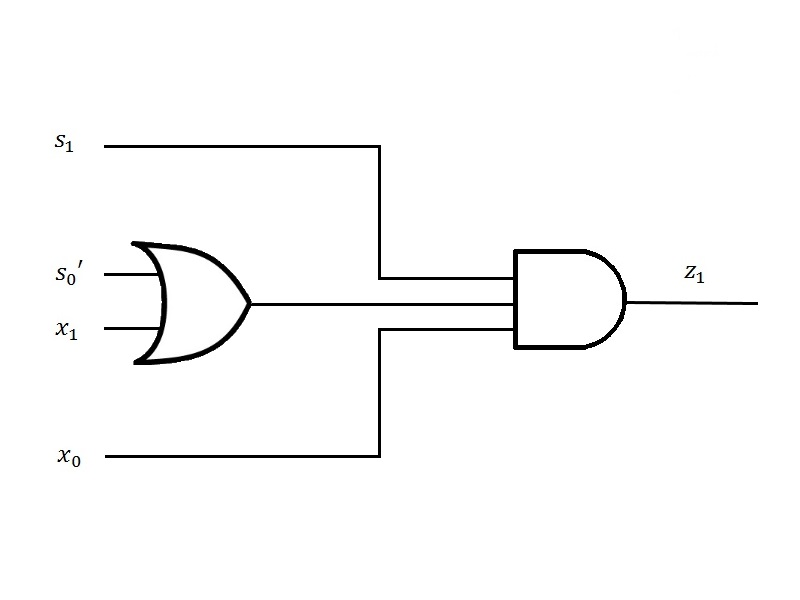
\includegraphics[scale=0.3]{z1}
\end{figure}

\begin{equation*}
z_1 = (s_1)(x_1)(s'_0)
\end{equation*}
\begin{figure}[h!]
\centering
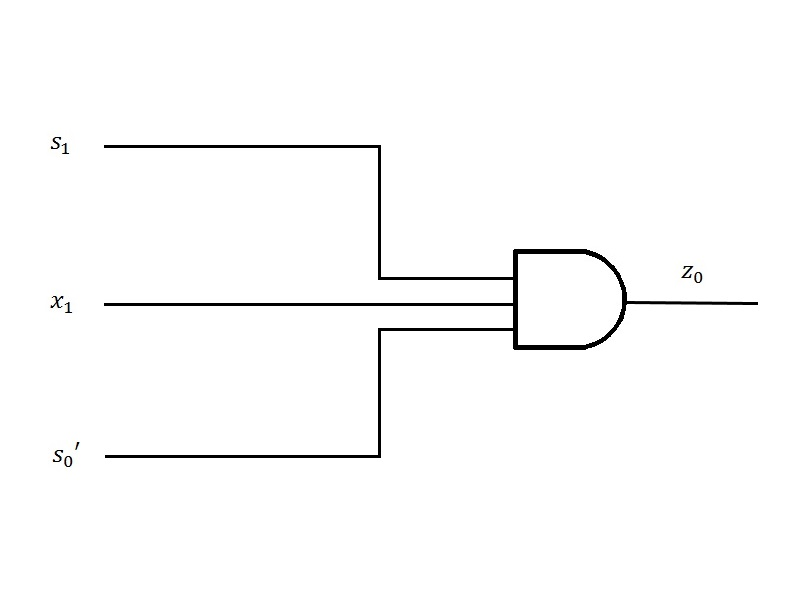
\includegraphics[scale=0.3]{z0}
\end{figure}

\clearpage

\begin{equation*}
J_1 = (x_0)(s_0 + x_1)
\end{equation*}
\begin{figure}[h!]
\centering
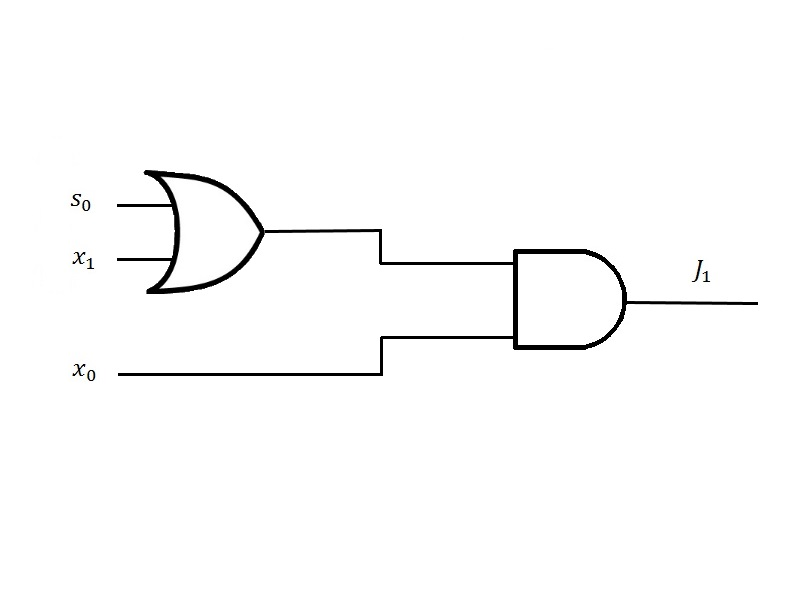
\includegraphics[scale=0.3]{J1}
\end{figure}

\begin{equation*}
K_1 = (x_0)(s'_0 + x_1)
\end{equation*}
\begin{figure}[h!]
\centering
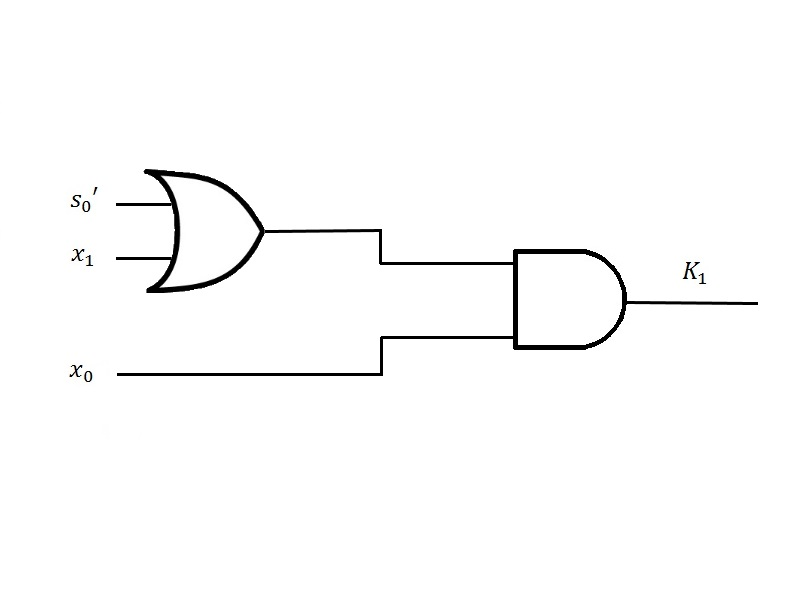
\includegraphics[scale=0.3]{K1}
\end{figure}

\clearpage

\begin{equation*}
J_0 = (s'_1)(x_0)
\end{equation*}
\begin{figure}[h!]
\centering
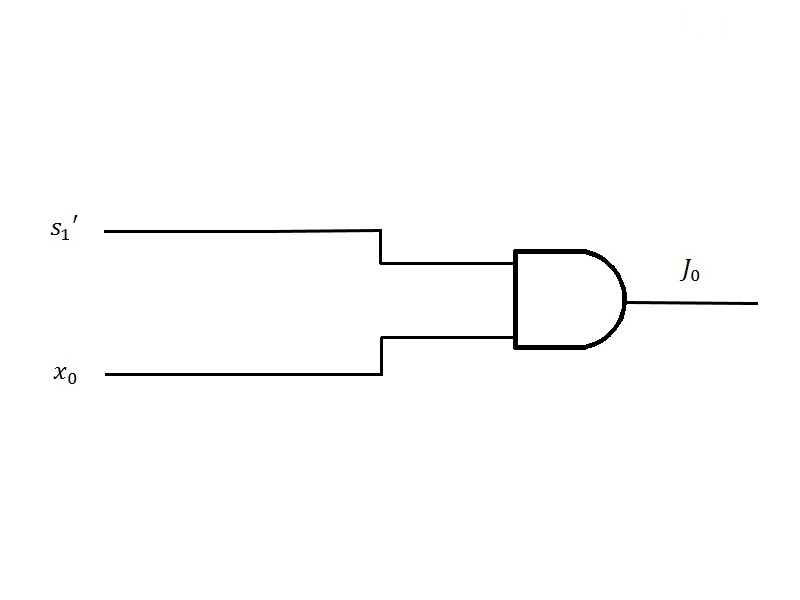
\includegraphics[scale=0.3]{J0}
\end{figure}

\begin{equation*}
K_0 = (x_0)(s_1 + x_1)
\end{equation*}
\begin{figure}[h!]
\centering
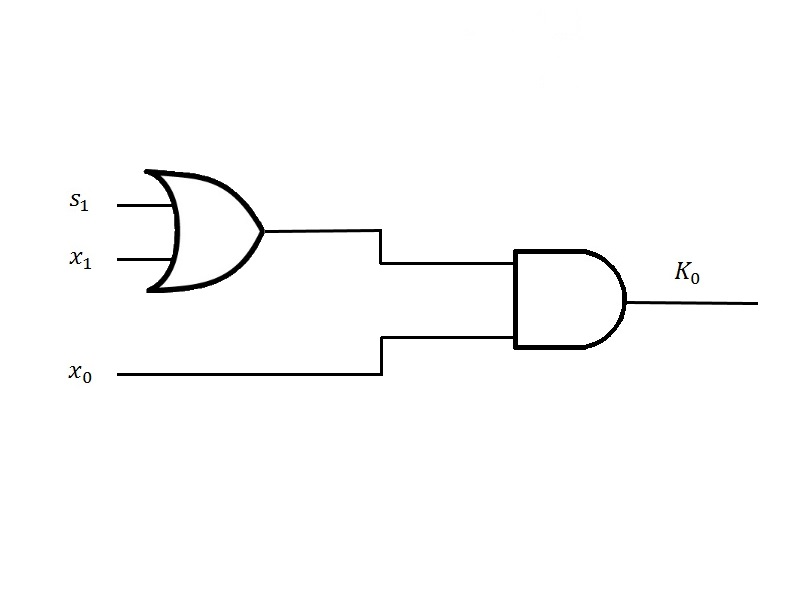
\includegraphics[scale=0.3]{K0}
\end{figure}

\textbf{We implemented negated inputs (of $s_0$ and $s_1$) as can be seen in
the overall network in the Appendix.}
The same expressions can also be found in the Appendix. The Appendix gives a 
step-by-step procedure to obtain those expressions.

%----------------------------------------------------------------------------
%	VERILOG CODE
%----------------------------------------------------------------------------

\section{Verilog Code}
The following is the implementation of our module in code, pasted from a 
Verilog file. Please also refer to \textit{csm51a\_proj3.v} in the zipped 
file.\\

\begin{verbatim}
Place implementation of code here.
\end{verbatim}

%----------------------------------------------------------------------------
%	SIMULATION RESULT
%----------------------------------------------------------------------------

\section{Simulation Result}
In your simulation, you should show the following 3 sequences: (1) D, N, D;
(2) N, N, N, N, and (3) D, Reset. Please clearly write down the necessary 
information on the waveform diagram so that one of your colleagues who does 
not know anything about your project could understand the behavior of the 
system you are trying to implement.\\

The following test bench code was used to generate that simulation result.

\begin{verbatim}
Place test bench code here.
\end{verbatim}

To observe the output values of each input combination, we changed the input 
every 10 nanoseconds.

%----------------------------------------------------------------------------
%	DESIGN REVIEW
%----------------------------------------------------------------------------

\section{Design Review}
This section includes a summary of your experiences throughout the project. 
It should be no more than TWO pages and may include such topics as what you 
have learned, problem(s) encountered during the implementation and the 
workarounds you came up with, the approach you used, the most important aspects 
of the project for you, where you spent most of the your time and suggestions 
you want to make. In particular, you may include here the new design scheme 
you proposed for the \textit{iKonPlus} controller and alternative 
implementation with MUXes for extra points.

%----------------------------------------------------------------------------
%	TEAM MEMBER CONTRIBUTIONS
%----------------------------------------------------------------------------

\section{Team Member Contributions}
In this section, a detailed description on each team member's responsibility 
and contribution should be presented clearly, including an estimate of 
percentage of efforts on the project and a summary list of each member in the 
project.

%----------------------------------------------------------------------------
%	APPENDIX
%----------------------------------------------------------------------------

\section{Appendix}
This part must show the complete worksheet during the paper-and-paper design.

\subsection{Inputs, Outputs, and States of the System}
Professor Yutao He always reminds his students to draw "The Box" when starting 
to design and analyze a digital system. Remembering that piece of advice, we 
started our design by drawing it to get a sense of the inputs and outputs. 
Those inputs and outputs are depicted in Figure~\ref{fig:box}. \\

\clearpage

\begin{figure}[h!]
\centering
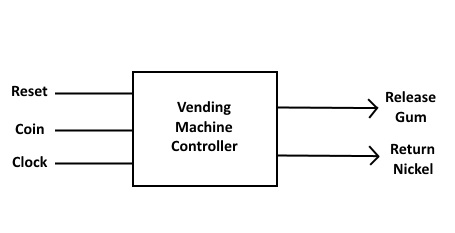
\includegraphics[scale=0.7]{Box}
\caption{"The Box!"}
\label{fig:box}
\end{figure}

The following tables show the inputs, outputs, and states of the \textit{iKon} 
Controller.

\begin{table}[h]
\begin{center}
\begin{tabular}{|c|c|c|c|l}
\cline{1-4}
\multicolumn{2}{|c|}{ \textbf{Inputs} } & 
\multicolumn{2}{c|}{ \textbf{Outputs} } &  \\ \cline{1-4}
  \textbf{Variables} & \textbf{Values} & \textbf{Variables} & \textbf{Values} &
  \\ \cline{1-4}
  Reset & \{True (T), False (F)\} & Release Gum (RG) & \{T, F\} &  \\
  Coin & \{ Empty (E), Nickel (N), Dime (D) \} & Return Nickel (RN) & \{T, F\} 
  &  \\ \cline{1-4}
\end{tabular}
\caption{The Inputs and Outputs of the \textit{iKon} Controller}
\end{center}
\end{table}

%\clearpage

\begin{table}[h]
\begin{center}
\begin{tabular}{|c|c|}
\hline
\textbf{State} & \textbf{Description}                  \\ \hline
Init           & Initial State                         \\
5c             & Amount of deposited coins is 5 cents  \\
10c            & Amount of deposited coins is 10 cents \\
15c            & Amount of deposited coins is 15 cents \\ \hline
\end{tabular}
\caption{The States of the \textit{iKon} Controller}
\end{center}
\end{table}


\subsection{Encoding Schemes}
Thee following tables show the encoding schemes that we used to design the 
sequential network.

\begin{table}[h]
\begin{center}
\begin{tabular}{cc|cc}
\textbf{Coin} & $x_1$$x_0$ & \textbf{Reset}       & r                    \\ \hline
Empty         & 00   & False                & 0                    \\
Nickel        & 01   & True                 & 1                    \\
Dime          & 11   & \multicolumn{1}{l}{} & \multicolumn{1}{l}{}
\end{tabular}
\caption{The Encoding Scheme of the Inputs}
\end{center}
\end{table}

\begin{table}[h]
\begin{center}
\begin{tabular}{cc|cc}
\textbf{RG} & $z_1$ & \textbf{RN} & $z_0$ \\ \hline
False       & 0  & False       & 0  \\
True        & 1  & True        & 1 
\end{tabular}
\caption{The Encoding Scheme of the Outputs}
\end{center}
\end{table}

\clearpage

\begin{table}[h]
\begin{center}
\begin{tabular}{c|c}
\textbf{State} & $s1$$s0$ \\ \hline
Init           & 11   \\
5c             & 01   \\
10c            & 11   \\
15c            & 10  
\end{tabular}
\caption{The Encoding Scheme of the States}
\end{center}
\end{table}


\subsection{State Diagram and State Table}
The following is the state diagram.

\begin{figure}[h!]
\centering
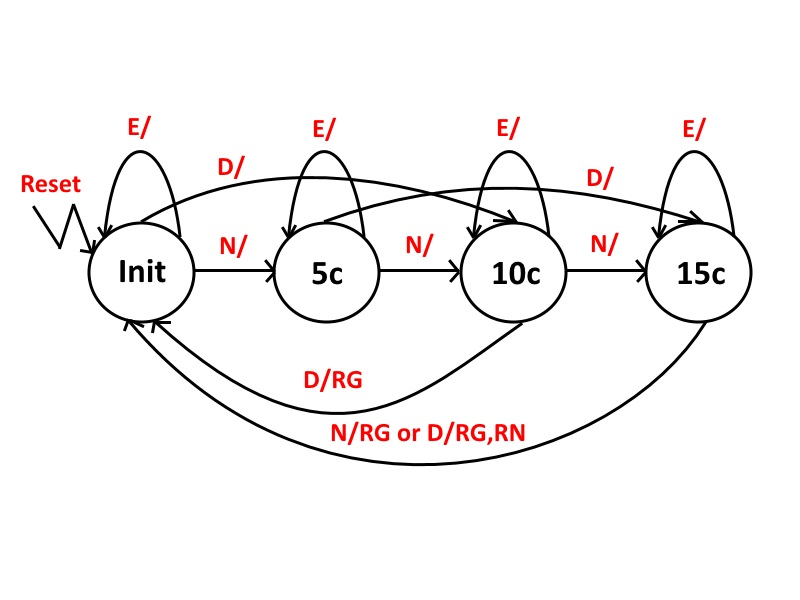
\includegraphics[scale=0.5]{State_Diagram}
\caption{The State Diagram of the Controller}
\end{figure}

The following is the state table obtained from the state diagram.
\clearpage

\begin{table}[h]\
\begin{center}
\begin{tabular}{c|ccc}
PS  & \multicolumn{3}{c}{ 
  \begin{tabular}[c]{@{}c@{}} Input \\ $x_1$$x_0$ 
  \end{tabular} 
} \\ \hline
s(t) = $s_1$$s_0$  & 00              & 01               & 11    \\ \hline
00                 & 00, 00          & 01, 00           & 11, 00\\
01                 & 01, 00          & 11, 00           & 10, 00\\
11                 & 11, 00          & 10, 00           & 00, 10\\
10                 & 10, 00          & 00, 10           & 00, 11\\ \hline
\multicolumn{1}{l|}{} & \multicolumn{3}{c}{
  \begin{tabular}[c]{@{}c@{}} NS, Output\\ s(t + 1), z = $z_1$$z_0$
  \end{tabular}
}
\end{tabular}
\caption{The State Table of the Controller}
\end{center}
\end{table}


\subsection{Minimization Procedure}
We used K-maps to find the minimal product of sums. The red circles in the 
K-maps shown below indicate the implicates used in the minimal expressions.\\

\begin{table}[h!]
\begin{tabular}{ c c }
\centering
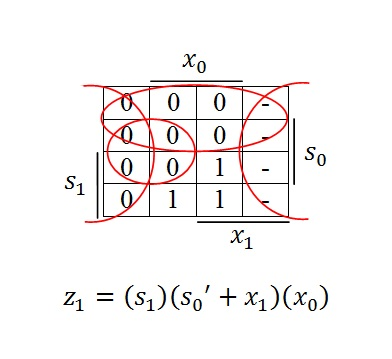
\includegraphics[scale=0.6]{z1-KMap} &
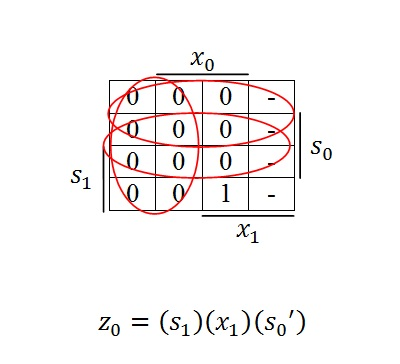
\includegraphics[scale=0.6]{z0-KMap} \\
\end{tabular}
\end{table}

\pagebreak

\begin{table}[h!]
\begin{tabular}{ c c }
\centering
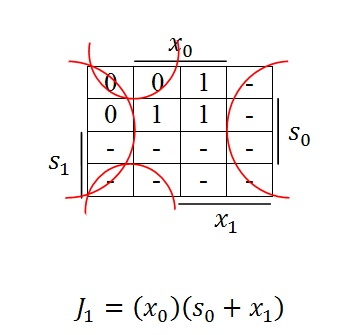
\includegraphics[scale=0.6]{J1-KMap} &
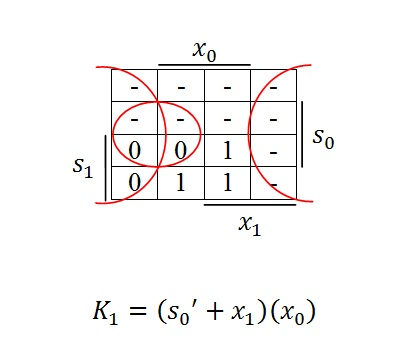
\includegraphics[scale=0.6]{K1-KMap} \\
\end{tabular}
\end{table}

\begin{table}[h!]
\begin{tabular}{ c c }
\centering
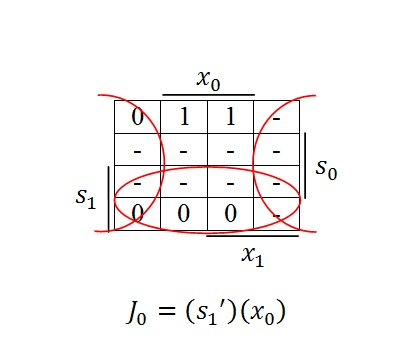
\includegraphics[scale=0.6]{J0-KMap} &
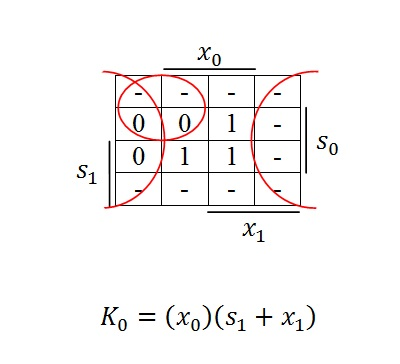
\includegraphics[scale=0.6]{K0-KMap} \\
\end{tabular}
\end{table}

\pagebreak


\subsection{Final Minimal Expressions}
After drawing the K-maps (from the previous section), we got the following 
minimal switching expressions in OR-AND form.\\

\begin{equation*}
z_1 = (s_1)(s'_0 + x_1)(x_0)
\end{equation*}

\begin{equation*}
z_1 = (s_1)(x_1)(s'_0)
\end{equation*}

\begin{equation*}
J_1 = (x_0)(s_0 + x_1)
\end{equation*}

\begin{equation*}
K_1 = (x_0)(s'_0 + x_1)
\end{equation*}

\begin{equation*}
J_0 = (s'_1)(x_0)
\end{equation*}

\begin{equation*}
K_0 = (x_0)(s_1 + x_1)
\end{equation*}

\clearpage

Combining each individual subnetwork of logic gates, we get the following 
circuit design.

\begin{figure}[h!]
\centering
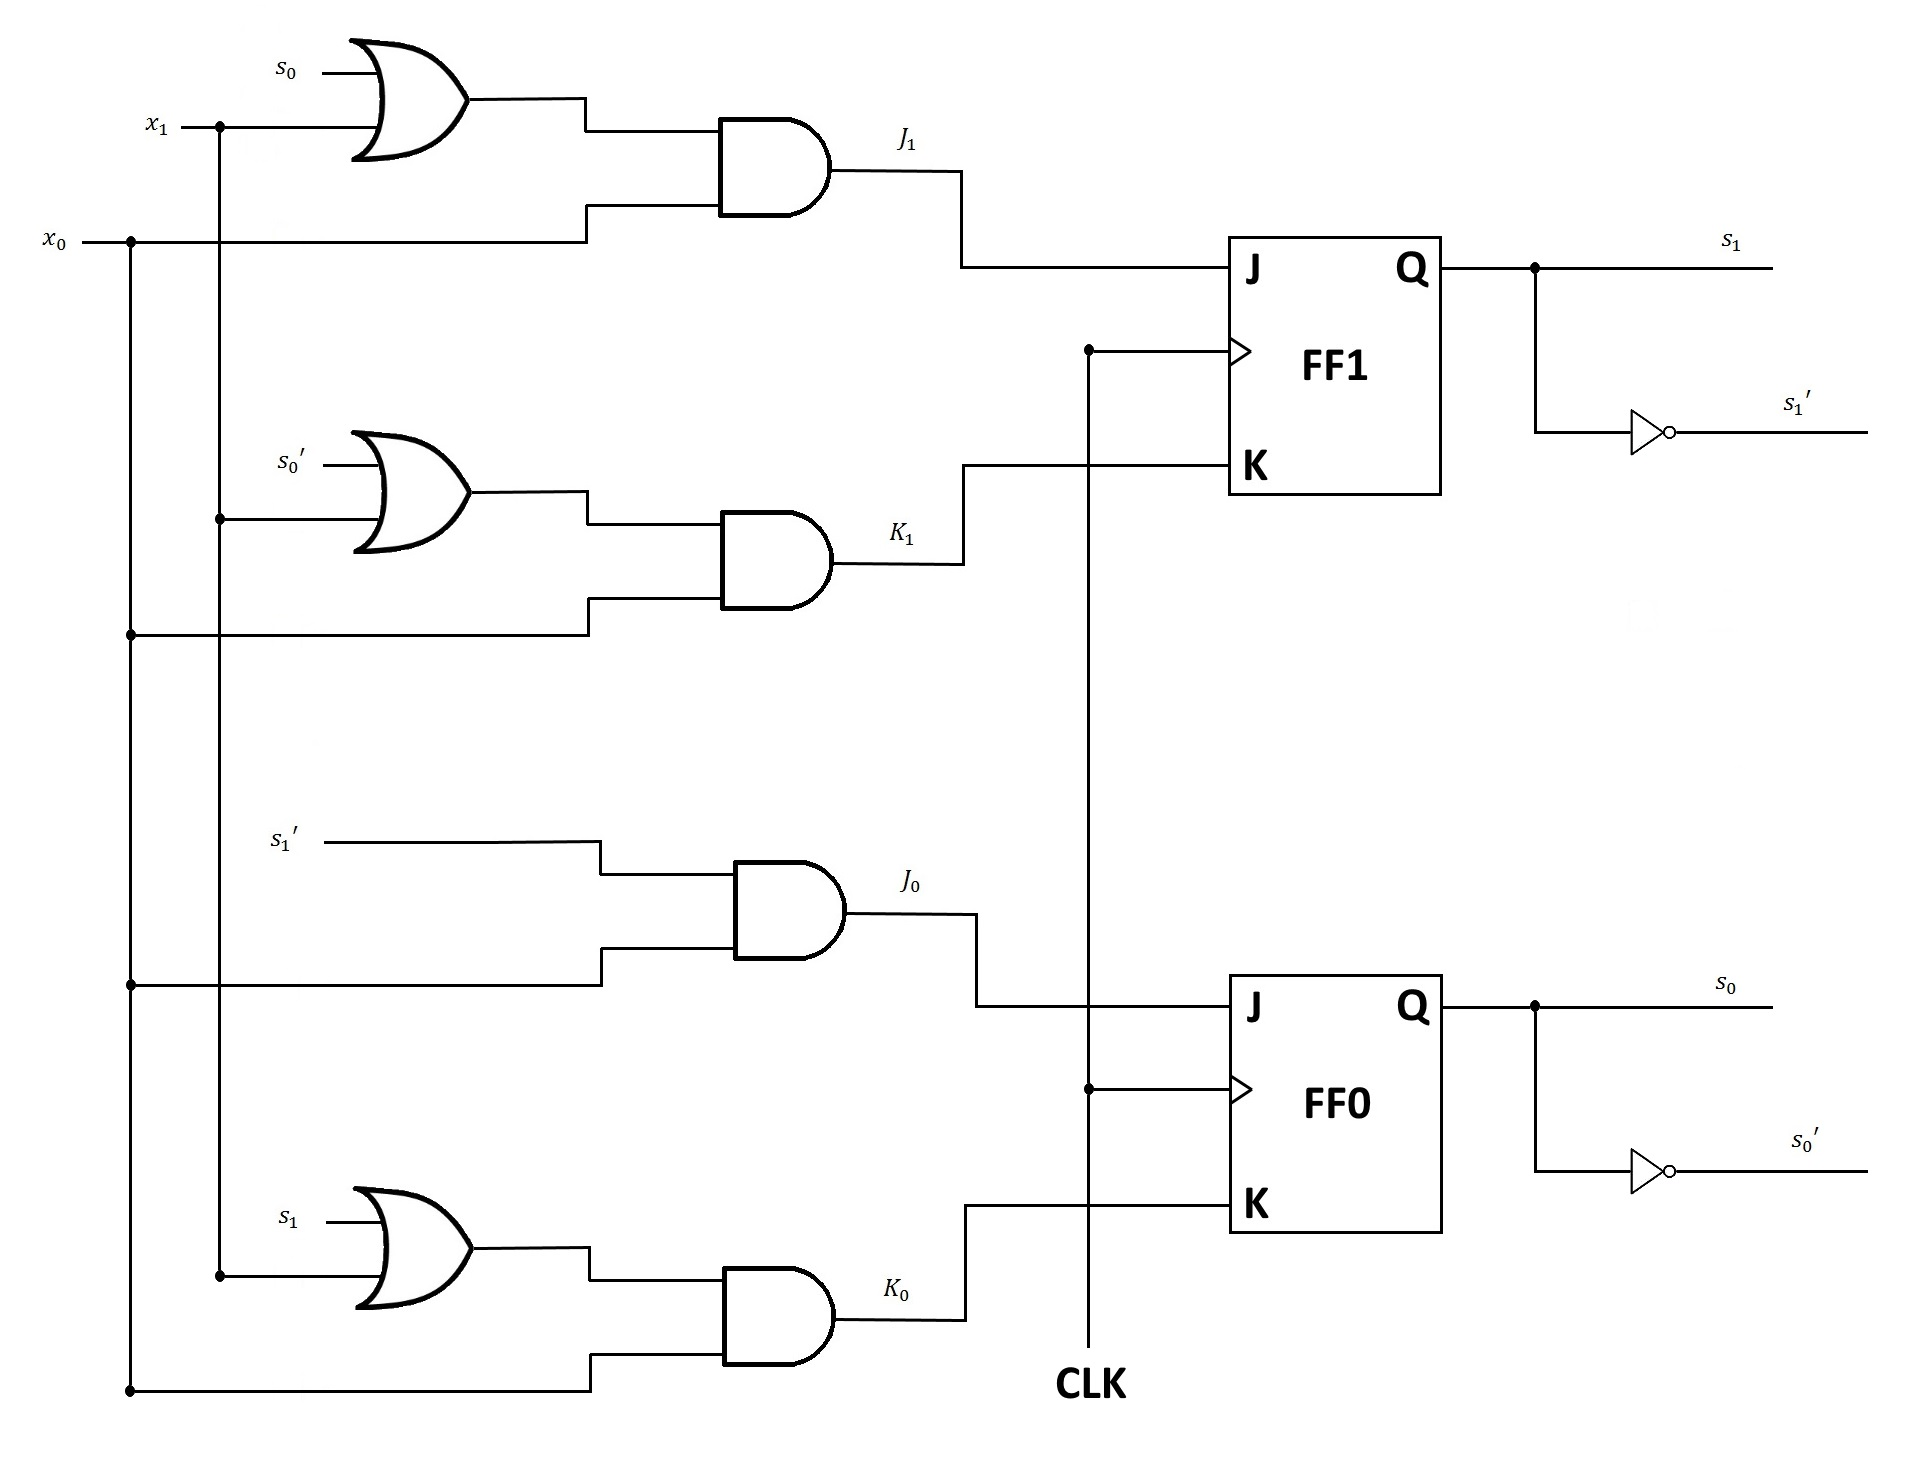
\includegraphics[scale=0.3]{Network}
\end{figure}

\begin{table}[h!]
\begin{tabular}{ c c }
\centering
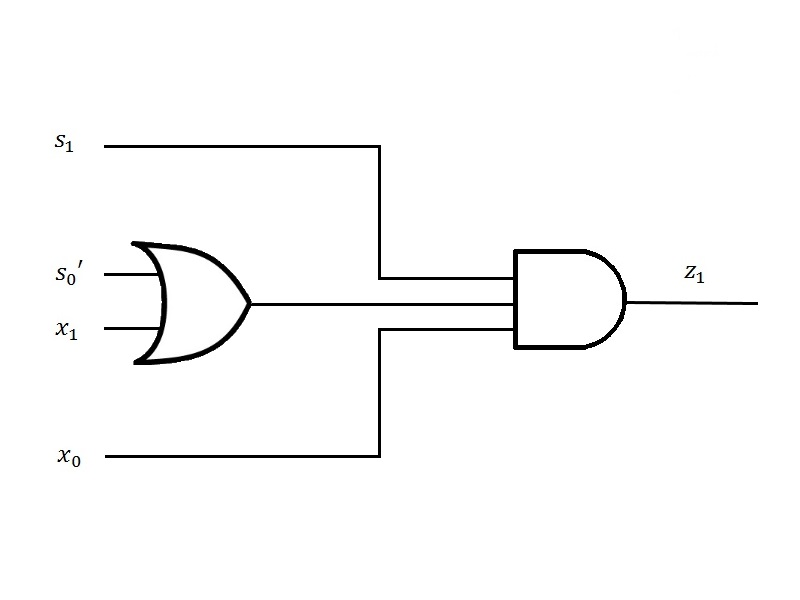
\includegraphics[scale=0.3]{z1} &
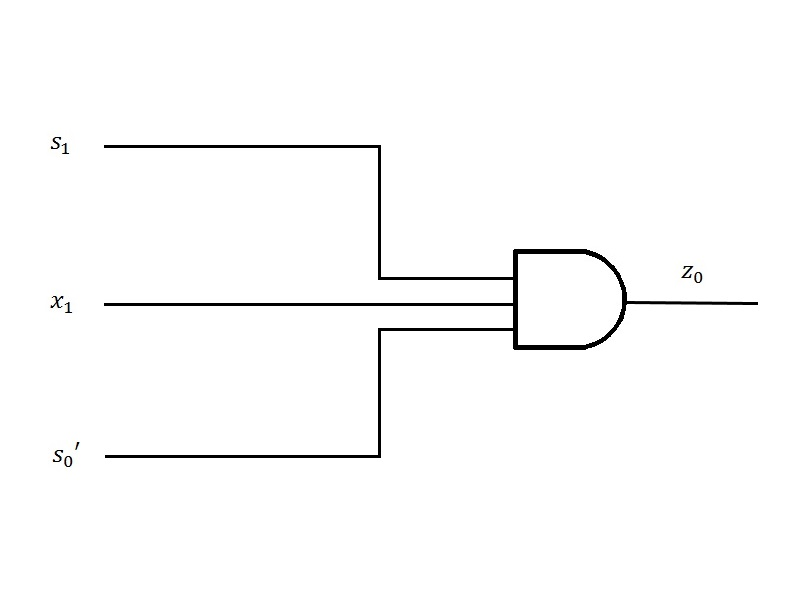
\includegraphics[scale=0.3]{z0} \\
\end{tabular}
\end{table}


\subsection{Paper-and-Pencil Design}
The following screenshots show our preliminary work done using paper and 
pencil.

%----------------------------------------------------------------------------
\end{document}